\documentclass[crop,tikz]{standalone}% 'crop' is the default for v1.0, before it was 'preview'
% %\usetikzlibrary{...}% tikz package already loaded by 'tikz' option
\usetikzlibrary{calc,patterns,angles,quotes}
\begin{document}
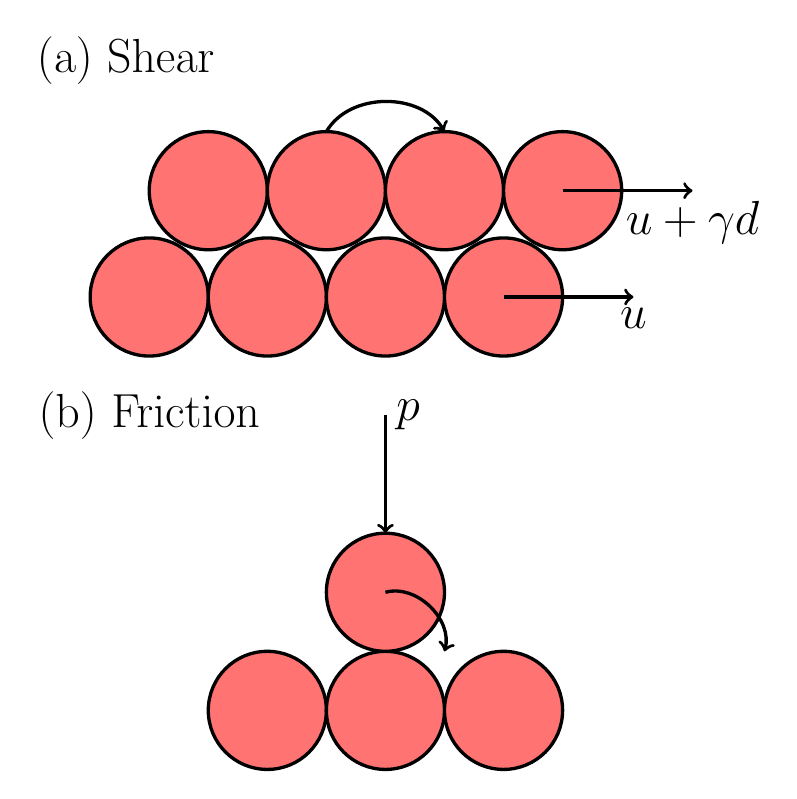
\begin{tikzpicture}[scale = 1.5]
    % \draw (-11.5,4) node {\textbf{A}};
    % \draw (-1.5,4) node {\textbf{B}};

    \def \b {3.5};
    \def \c {-7};
    \def \d {0.1};
    \def \r {0.5};
    \node at (1.8, 3)  {\LARGE (a) Shear};
    % Before dilatancy
    \foreach \x in { 2, 3, 4, 5}
        \foreach \y in {1}
            \draw [color=black, fill=red!55,very thick] (\x, \y) circle (0.5);

    \foreach \x in { 2.5, 3.5, 4.5, 5.5}
        \foreach \y in {1.9}
            \draw [color=black, fill=red!55,very thick] (\x, \y) circle (0.5);
            
    \draw[->, very thick] (5, 1) -- (6.1, 1) node[below] {\LARGE $u$};
    \draw[->, very thick] (5.5, 1.9) -- (6.6, 1.9) node[below] {\LARGE $u + \gamma d$};
    \draw[->, very thick, black] (3.5, 2.4) to [bend left=60] (4.5,2.4);

    \node at (2, 3.5-\b)  {\LARGE (b) Friction};
    % Before dilatancy
    \foreach \x in { 3, 4, 5}
        \foreach \y in {1-\b}
            \draw [color=black, fill=red!55,very thick] (\x, \y) circle (0.5);

            \draw [color=black, fill=red!55,very thick] (4, 2-\b) circle (0.5);
            

    \draw[->, very thick, black] (4, 2-\b) to [bend left=60] (4.5,1.5-\b);
    \draw[->, very thick] (4, 3.5-\b) node[right] {\LARGE $p$}  -- (4, 2.5-\b) ;


\end{tikzpicture}
\end{document}